\chapter{Literature Review}%
\label{chapter:literatureReview}

\begin{introduction}
In the chapter II will cover the review the literature about the context of this dissertation, that include the vehicle maintenance and the service quality at the dealerships. 
Additionally, I will also present a small background of the LightMobie Company and an analysis of the available architecture to implement the software solution.
\end{introduction} 


To acquire information about this topic I search information on the platform Scopus and Google Scholar. 
In Scopus, I used multiple queries, the first one was \"Vehicle AND Maintenance AND dealerships\" and found 49 papers.
On a primarly analysis from the title and abstract i selected 24 papers that were related to this topic.
However, on a further examination, I chose to write about 3 papers in this pre-dissertation. 
Most of the papers i discarded was because of the use of the words \"Vehicle\" and \"dealerships\". 
This words made the search return the papers that envisioned the dealerships as a reselling unit of the main company, which is not the focus of this dissertation.
Another reason was the use of machine learning to solve a specific problem, like predictive maintenance. 
The two papers i write in this dissertation were chosen because two was a research study about the process of vehicle maintenace and explain the importance of a quality of service in this industry.
In the other paper, the authors describe a solution implementation of a vehicle maintenace service for a dealership in Africa, which is exacly the use case of this dissertation.
In google scholar i found 3 papers about the electric vehicle in China. 
They may be important because if we can understand the market in another country, the company can expand its business (vehicle sharing) to that country and in turn surge the need for dealerships to arise.
However i chose to not include in this pre-dissertation.  
The three papers i write in this dissertation were chosen because two of them were research studies about the process of vehicle maintenace and explain the importance of a quality of service in this industry.
The other paper described a solution implementation of a vehicle maintenace service for a dealership in Africa, which is exacly the use case of this dissertation.
With this three papers i could give a definition of the context and aquire some problems and solutions to focus on in the development fase.  



% \section{Background}

% The LightMobie is a company stablished in Águeda that provides a diverse set of products in the shared mobility sector. 
% The company also provides a software system to integrate with their bicycles and stations and vehicle maintenance.
% Currently, the company is in step of renewal of the system to a new solution of the bicycles and stations and is building a platform to interact and manage that system.
% This platform is able to visualize current and past information of the vehicle, stations and users and there interaction with each other.
% Additionally, alerts triggered by the equipment are also visible in the dashboard and the user can elaborate statistics on this data.

\section{Vehicle Maintenance}

Delivering vehicle maintenance services involves numerous activities, each crucial for maintaining service quality and ensuring customer satisfaction. 
Any deviation from these activities can negatively impact quality, leading to dissatisfaction. 
The dissatisfaction of a client reduces their loyalty to company, wich can lead to a decrease in the number of clients and a decrease in revenue. ~\cite{Setting_the_after_sale_process}
To mitigate this Quality Control must supervise every stage of the process—from scheduling appointments to repairs and final vehicle delivery. ~\cite{Setting_the_after_sale_process}

The macro-level flow of a vehicle maintenance or repair service is illustrated in the figure \ref{fig:Vehicle_maintenace_macro}. 




\begin{figure}[h]
  \caption{Macro-level Flow of a vehicle maintenance or repair service. This figure was inspired by figure 6: After Sales process from ~\citet{Setting_the_after_sale_process}.}
  \centering
  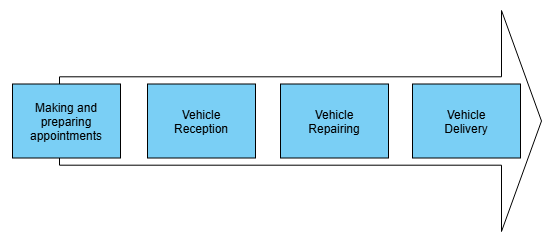
\includegraphics[width=0.50\textwidth]{figs/Vehicle_maintenace_macro}
  \label{fig:Vehicle_maintenace_macro}
\end{figure}


The first step of the process starts with a client interacting with the garage to schedule a maintenance or repair. 
After that, the client goes to the garage and the receptionist receives the client and the vehicle.
Then the mechanic will perform the maintenance or repair on the vehicle.
And, Finally, the client will receive the vehicle back from the garage.

To ensure quality in the first step the receptionist must understand the fill capacity of the garage and the time to complete the job. 
This step is very important because a mistake can lead to a break of promisses for the organization. ~\cite{Setting_the_after_sale_process}
The second step the receptionist and service advisor, when receiving the vehicle, must do a visual confirmation of the vehicle condition. ~\cite{Setting_the_after_sale_process}
Explain to the client the services of the garage and their prices. Agree with the client the services to be performed and the time to complete the job. 
Then receptionist insert into the system this information. ~\cite{Setting_the_after_sale_process}

Following beguins the third step and most important fase, the mechanic will perform the maintenance or repair on the vehicle. 
In this process, the quality control must supervise all the proccess to ensure that the job is done correctly. ~\cite{Setting_the_after_sale_process}
This includes the repair process, extra work, final tests, vehicle wash, service report and promissed date and delivery. ~\cite{Setting_the_after_sale_process}
To accomplish that the use of a checklist is recommended to ensure precision and accuracy at each step. ~\cite{Setting_the_after_sale_process}

Finally, the last step is the delivery of the vehicle to the client. 
In here  the admin must review the work done and the final price of the service, to avoid unnecessary payments from the client and not paying the workers for the done work. ~\cite{Setting_the_after_sale_process}

with this the a vehicle maintenance is completed with quality. 
But how do you measure the quality of the service?
I will address that in the next section.

\section{Service Quality}
The concept of service quality is well-documented, with the SERVQUAL model being among the most recognized modules. 
SERVQUAL, in particular, provides a multidimensional approach for comparing consumers' perceptions of service quality against their expectations. 
It emphasizes five core dimensions ~\cite{SERVQUAL_OLD}:

\begin{itemize}
  \item Tangibles – Physical facilities, equipment, and appearance of personnel.
  \item Reliability – Ability to consistently deliver services as promised.
  \item Responsiveness – Willingness to assist the customer and proactivity.
  \item Assurance – Demonstrate courtesy and knowledge and inspire trust and confidence.
  \item Empathy – Caring and treat customers as individuals.
\end{itemize}

To measure the quality of the service one needs to do a questionnaire composed of 22 questions that are divided into the five dimensions of the SERVQUAL model. ~\cite{Measuring_After_sales_Service_Quality}
Each question must be divided into two answers, the first one is a score of the expectation of the service provided and the second one is the perception of the service. ~\cite{Measuring_After_sales_Service_Quality}
In some cases is recommended to do two interviews with the same client, one before the service to aquire the expectations and another after the service to aquire the perception. ~\cite{servqual_blog_da_qualidade}
The difference between the two answers is the quality of the service. ~\cite{servqual_blog_da_qualidade} ~\cite{Measuring_After_sales_Service_Quality} ~\cite{SERVQUAL_OLD}

In the paper of ~\cite{Measuring_After_sales_Service_Quality} the authors used the SERVQUAL model to measure the quality of the service at a CMV SA dealership in South Africa.
The authors collected the data from a semi-structured questionnaire and interviews with customers, managers, and staff.
The questionnaire was composed of 22 statements that can be seen in the figure \ref{fig:SERVQUAL_results} where the respondent used the Likert's point scale ranging from 1 (strongly disagree) to 5 (strongly agree) to rate the expectation and perception of each individual item.
With this answers the authors measured the service quality by calculating the difference of the scores between each item.
 
\begin{figure}[h]
  \caption{SERVQUAL statements used by the authors in the study to measure the quality of the service at a CMV SA dealership in South Africa (~\cite{Measuring_After_sales_Service_Quality}).}
  \centering
  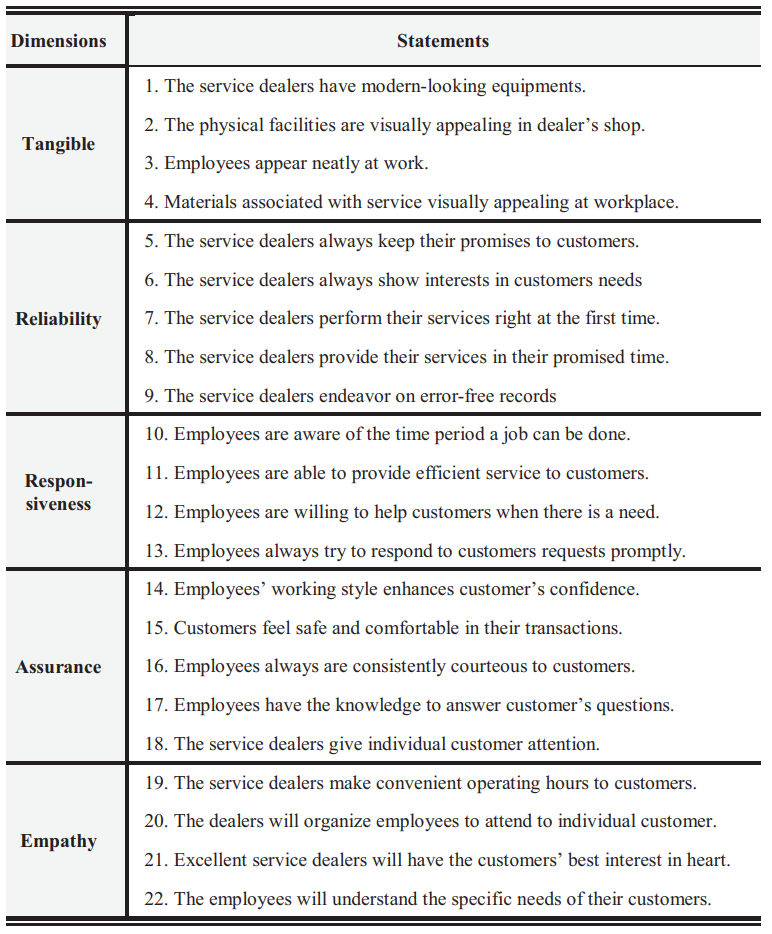
\includegraphics[width=0.50\textwidth]{figs/SERVQUAL_statements}
  \label{fig:SERVQUAL_statements}
\end{figure}


The results seen in figure \ref{fig:SERVQUAL_results} revealed a negative score in all five dimensions of the SERVQUAL model. 
Even comparing the expectation of the customers with the expectation of the dealers the average score was negative (-0.10).
This shows that the services provided by the CMV SA dealer are not meeting the expectations of the customers according to the SERVQUAL five dimensions.
The customer also give some recommendations gather in the interviews done after the questionnaire. 
They include opening more workshops to reduce travel inconvenience and ensuring timely parts availability.
The authors also recommend that the dealer should conduct regular SERVQUAL assessments to monitor and address service quality gaps and emphasize the importance of the service quality tom maintain competitiveness and drive long-term business success. ~\cite{Measuring_After_sales_Service_Quality}


\begin{figure}[h]
  \caption{SERVQUAL results of the study to measure the quality of the service at a CMV SA dealership in South Africa. In the table the header \"Exp\" means the expectation, \"Per\" means the perception, \"Zc\" means the Service quality score from the customers and the \"Zc-ms\" means Service quality score measure by the difference of the expectations of the customer and the expectation of the dealers. (~\cite{Measuring_After_sales_Service_Quality})}
  \centering
  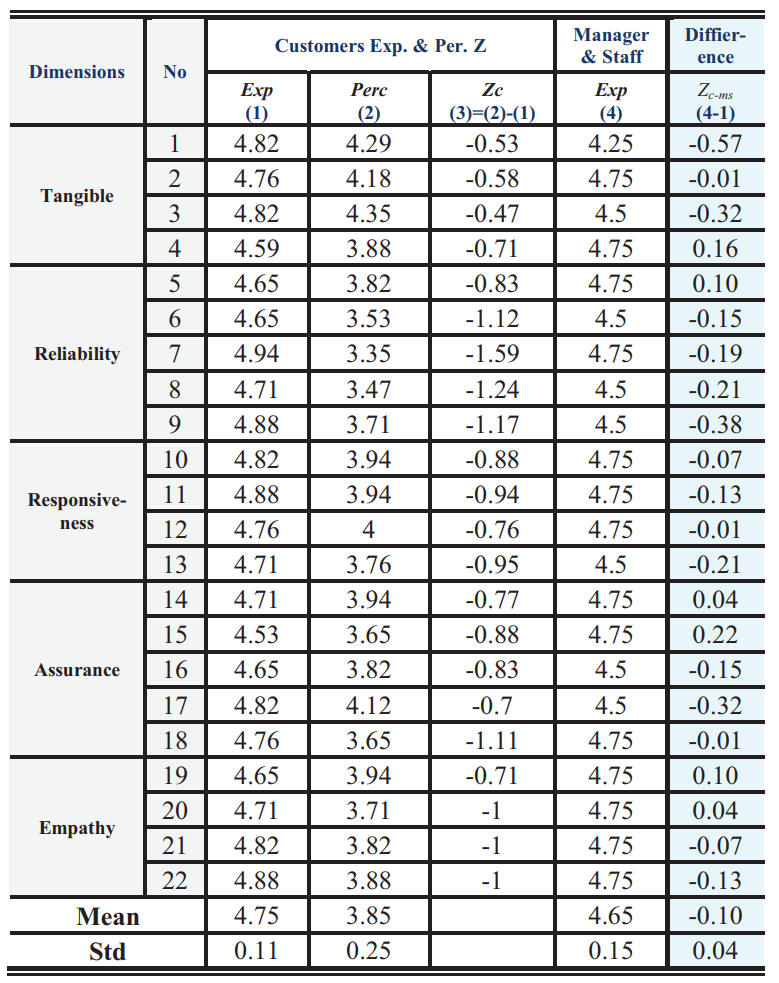
\includegraphics[width=0.75\textwidth]{figs/SERVQUAL_results}
  \label{fig:SERVQUAL_results}
\end{figure}

% \section{Increase Clients Satisfaction in Vehicle Maintenance}
% In belgrade, serbia, in 2013, a research was conducted to measure the satisfaction of the clients at dealerships. ~\cite{Setting_the_after_sale_process}
% In the reasearch, they divided the consumers' expectations or demands in three categories:
% \begin{itemize}
%   \item quality of repair work, service done within the agreed time schedule, price, friendliness and professionalism, the time waiting for an appointment. 
%   \item availability of spare parts, advice given for further maintenance, information given about additional work. 
%   \item adequate documentation about accomplished work, replacing vehicles, to invoices explained, café, Wi-Fi, phone availability. In this paper only the first category has been taken into consideration. 
% \end{itemize}



% The GAP model, precedent from the SERVQUAL, also measures service quality by identifying the difference between customer expectations and actual perceptions. 
% These gaps include discrepancies between customer expectations and management's understanding, management's perceptions and service specifications, service specifications and actual delivery, actual delivery and communicated services, and expected and delivered service. ~\cite{Measuring_After_sales_Service_Quality}

% https://forms.app/en/blog/gap-model-of-service

\section{Service Management for MAS Motors LLC}

MAS Motors LLC is a Toyota dealership that provides vehicle maintenance services in Libya.
This company handles the daily work manually using basic applications, word documents and paper documents.
This causes accidental human errors, which in turn lead to the managers' intuition to make a decision based on the data.
This old approach is inefficent with the expand of the business and the company needs a more modern method to handle the huge amount of work and achieve continuous success. ~\cite{MAS_MOTORS}
So the author of the paper developed a web application that facilitates and increase the performance of the work at the dealership.
The system targets multiple user groups, such as service advisers, technicians, and customers, and offers a centralized platform to manage tasks like job card management, inventory updates, and customer service. ~\cite{MAS_MOTORS}
The authors' application was developed using the Laravel, which is a PHP web application framework, with MariaDB as the database management system, which is a popular open source relational database.

They applied \ac{RAD} methodology as a software development tool to develop the application.
\ac{RAD} is an agile software development approach that focuses on rapid prototyping and quick feedback from users over a costly planning. ~\cite{rapid_app_development}
This appreoach ideology is an ongoing testing and refinement of the project instead of following a detailed planning and design such as traditional models.
It is composed of four phases: Define requirements, prototype, feedback, and final product. ~\cite{rapid_app_development}
In the requirement phase is defined by the definition of an unrestricted set of requirements, that can be changed during any point in the cycle. 
In the prototype phase, the developers create a prototype of the system to Demonstrate to the client. 
This prototype may be rushed since in the finalization stage, the developers will refine the final product. ~\cite{rapid_app_development}
In the next phase, the feedback, developers present their work to the client and end-users.
Depending on the feedback, the client want to change the requirements or add something new. In this case, the developers will go back to the second stage and repeat the process. ~\cite{rapid_app_development}
On a positive feedback, the client is satisfied by the prototype and the developers will move to the final product phase.
In this final phase, the developers will refine the prototype by optimizing and re-engineer their implementation to improve stability and maintainability. ~\cite{rapid_app_development}
The authors of the paper chose this software development tool due to its feedback, flexibility and quickness.

For the first phase the authors write the requirements of the system following the Hewlett-Packard \ac{FURPS} model that categorize the software requirements into functional and non-functional aspects.
The acronym stands for:

\begin{itemize}
  \item Functionality – The core features and business-domain-specific aspects.
  \item Usability – User interface considerations like accessibility and aesthetics.
  \item Reliability – System availability, accuracy, and failure recovery.
  \item Performance – Metrics such as response time and throughput.
  \item Supportability – Testability, maintainability, and scalability.
\end{itemize}

The results of the application were positive, the survey response from employees and customers classified the system according to the \ac{FURPS} model with the scores 4.27 for functionality, 4.30 for usability, 4.27 for reliability, 4.46 for performance, and 3.36 for supportability.
Supportability was the lowest score, due to limited configuration options ~\cite{MAS_MOTORS}, however, the overall system imporved significantly the service efficiency and customer satisfaction. ~\cite{MAS_MOTORS}

The authors included some employee recommendations for future enhancements, such as SMS notifications for service reminders, integrating social media, and expanding customer configuration options.


\section{Architecture}

The architecture of the application will have a \ac{MVC} pattern. 
The \ac{MVC} pattern is a software design pattern that separates the application into three main components: Model, View, and Controller.~\cite{mvc_geeksforgeeks} ~\cite{MVC_StartupHouse}
The Model is responsable for the storage of data and the logic of the application.  ~\cite{mvc_geeksforgeeks} ~\cite{MVC_StartupHouse}
It provides an abstraction layer of the database that allows data operation without the direct contact from the user interface. ~\cite{MVC_StartupHouse}
It also controls the business logic of the application, such as calculations, data validation and data manipulation. ~\cite{MVC_StartupHouse}

The View represents the \ac{UI} of the application and is used to present the information from the Model component. ~\cite{mvc_geeksforgeeks} ~\cite{MVC_StartupHouse}
This component is also responsable for the user's interactions and it does not contain any logic of the application, only limits itself to the communication between the Controller and the user. ~\cite{MVC_StartupHouse}

The Controller acts as an intermediary between the Model and View.
It receives the user's input and it is responsable to process the data and update the Model based on the user's actions and update the view to give feedback of the changes maded. ~\cite{mvc_geeksforgeeks} ~\cite{MVC_StartupHouse}

This pattern is popular for designing designing applications because it provides a clean separation of concerns. This separation, increases the maintainability and reusability of the code, facilitates the creation of the test and turns the application more scalable. ~\cite{mvc_geeksforgeeks} ~\cite{MVC_StartupHouse}
The \ac{MVC} pattern is a popular pattern for designing applications because it provides a clean separation of concerns, making it easier to maintain and test the application. ~\cite{mvc_geeksforgeeks} ~\cite{MVC_StartupHouse}
This requirements are advantageous, since the functional requirements of the project are not fully stablished and may receive some suggestion from the company along the way. 
The scalability is also important since the aim market of this application are the company's dealerships that may be scattered across the country or even Europe.

The framework the application will be built with is the Asp Net Core MVC. 
I believe this approach will be better than following the successful application from \citet{MAS_MOTORS} for multiple reasons.
The integration with the microsoft framework MYSQL database is more simple when using ASP.NET Core due to the package Entity Framework [https://learn.microsoft.com/en-us/aspnet/entity-framework]. 
Laravel also supports this database interaction, but Asp Net Core MVC is more suitable for this environment. ~\cite{asp_net_vs_laravel}
Additionally, Laravel loses in performance with the Compiled Language ASP.NET since it is a Interpreted language. 
In security, larabel offers some security features like hashing or secure input validation, but requires deeper PHP knowledge and proactive vulnerability management. 
Microsoft offers greater security tools that provides a major abstraction to this concept and allows the develop to focus on the application functionalities. ~\cite{asp_net_vs_laravel}

Despite all of this advantages, the main reason to use this framework and pattern is to integrate with the Fleet Management System that has the same approach. 
Since i was involved in the project i am familiar with this technology, so, even though ASP.NET can have a greater learning curve for unfamiliar developers ~\cite{asp_net_vs_laravel}, I am not in that category.

Based on the feedback from the users in the study from ~\citet{MAS_MOTORS}, where the authors refer a integration of a SMS notification system to remind customers of scheduled visits, i decided to integrate to this platform another application for the customers. 
This application functionality is to notify the user about the progress of the maintenance and get feedback for the service provided at the dealership.
It has the purpose of increasing the user satisfaction by keeping the client inform and gather information about future improvements.
This application will be built as a \ac{PWA} in ASP.NET Core mvc, for convenience purpose and simplicity.

To summarize, I will develop 2 application in this dissertation in ASP.NET Core to be integrated in the developed system at Lightmobie, one for the workers at the dealership and another for their clients.







